
%% bare_conf.tex
%% V1.3
%% 2007/01/11
%% by Michael Shell
%% See:
%% http://www.michaelshell.org/
%% for current contact information.
%%
%% This is a skeleton file demonstrating the use of IEEEtran.cls
%% (requires IEEEtran.cls version 1.7 or later) with an IEEE conference paper.
%%
%% Support sites:
%% http://www.michaelshell.org/tex/ieeetran/
%% http://www.ctan.org/tex-archive/macros/latex/contrib/IEEEtran/
%% and
%% http://www.ieee.org/

%%*************************************************************************
%% Legal Notice:
%% This code is offered as-is without any warranty either expressed or
%% implied; without even the implied warranty of MERCHANTABILITY or
%% FITNESS FOR A PARTICULAR PURPOSE! 
%% User assumes all risk.
%% In no event shall IEEE or any contributor to this code be liable for
%% any damages or losses, including, but not limited to, incidental,
%% consequential, or any other damages, resulting from the use or misuse
%% of any information contained here.
%%
%% All comments are the opinions of their respective authors and are not
%% necessarily endorsed by the IEEE.
%%
%% This work is distributed under the LaTeX Project Public License (LPPL)
%% ( http://www.latex-project.org/ ) version 1.3, and may be freely used,
%% distributed and modified. A copy of the LPPL, version 1.3, is included
%% in the base LaTeX documentation of all distributions of LaTeX released
%% 2003/12/01 or later.
%% Retain all contribution notices and credits.
%% ** Modified files should be clearly indicated as such, including  **
%% ** renaming them and changing author support contact information. **
%%
%% File list of work: IEEEtran.cls, IEEEtran_HOWTO.pdf, bare_adv.tex,
%%                    bare_conf.tex, bare_jrnl.tex, bare_jrnl_compsoc.tex
%%*************************************************************************

% *** Authors should verify (and, if needed, correct) their LaTeX system  ***
% *** with the testflow diagnostic prior to trusting their LaTeX platform ***
% *** with production work. IEEE's font choices can trigger bugs that do  ***
% *** not appear when using other class files.                            ***
% The testflow support page is at:
% http://www.michaelshell.org/tex/testflow/



% Note that the a4paper option is mainly intended so that authors in
% countries using A4 can easily print to A4 and see how their papers will
% look in print - the typesetting of the document will not typically be
% affected with changes in paper size (but the bottom and side margins will).
% Use the testflow package mentioned above to verify correct handling of
% both paper sizes by the user's LaTeX system.
%
% Also note that the "draftcls" or "draftclsnofoot", not "draft", option
% should be used if it is desired that the figures are to be displayed in
% draft mode.
%
\documentclass[conference]{IEEEtran}
% Add the compsoc option for Computer Society conferences.
%
% If IEEEtran.cls has not been installed into the LaTeX system files,
% manually specify the path to it like:
% \documentclass[conference]{../sty/IEEEtran}


\usepackage[latin1]{inputenc}
\usepackage[T1]{fontenc}


% Some very useful LaTeX packages include:
% (uncomment the ones you want to load)


% *** MISC UTILITY PACKAGES ***
%
%\usepackage{ifpdf}
% Heiko Oberdiek's ifpdf.sty is very useful if you need conditional
% compilation based on whether the output is pdf or dvi.
% usage:
% \ifpdf
%   % pdf code
% \else
%   % dvi code
% \fi
% The latest version of ifpdf.sty can be obtained from:
% http://www.ctan.org/tex-archive/macros/latex/contrib/oberdiek/
% Also, note that IEEEtran.cls V1.7 and later provides a builtin
% \ifCLASSINFOpdf conditional that works the same way.
% When switching from latex to pdflatex and vice-versa, the compiler may
% have to be run twice to clear warning/error messages.

\usepackage[dvips]{graphicx}
\graphicspath{{figs-copie}}
\DeclareGraphicsExtensions{.eps}

\usepackage{amssymb,amsmath,array}

\usepackage{algorithm,algorithmic}


% *** CITATION PACKAGES ***
%
%\usepackage{cite}
% cite.sty was written by Donald Arseneau
% V1.6 and later of IEEEtran pre-defines the format of the cite.sty package
% \cite{} output to follow that of IEEE. Loading the cite package will
% result in citation numbers being automatically sorted and properly
% "compressed/ranged". e.g., [1], [9], [2], [7], [5], [6] without using
% cite.sty will become [1], [2], [5]--[7], [9] using cite.sty. cite.sty's
% \cite will automatically add leading space, if needed. Use cite.sty's
% noadjust option (cite.sty V3.8 and later) if you want to turn this off.
% cite.sty is already installed on most LaTeX systems. Be sure and use
% version 4.0 (2003-05-27) and later if using hyperref.sty. cite.sty does
% not currently provide for hyperlinked citations.
% The latest version can be obtained at:
% http://www.ctan.org/tex-archive/macros/latex/contrib/cite/
% The documentation is contained in the cite.sty file itself.






% *** GRAPHICS RELATED PACKAGES ***
%
\ifCLASSINFOpdf
  % \usepackage[pdftex]{graphicx}
  % declare the path(s) where your graphic files are
  % \graphicspath{{../pdf/}{../jpeg/}}
  % and their extensions so you won't have to specify these with
  % every instance of \includegraphics
  % \DeclareGraphicsExtensions{.pdf,.jpeg,.png}
\else
  % or other class option (dvipsone, dvipdf, if not using dvips). graphicx
  % will default to the driver specified in the system graphics.cfg if no
  % driver is specified.
  % \usepackage[dvips]{graphicx}
  % declare the path(s) where your graphic files are
  % \graphicspath{{../eps/}}
  % and their extensions so you won't have to specify these with
  % every instance of \includegraphics
  % \DeclareGraphicsExtensions{.eps}
\fi
% graphicx was written by David Carlisle and Sebastian Rahtz. It is
% required if you want graphics, photos, etc. graphicx.sty is already
% installed on most LaTeX systems. The latest version and documentation can
% be obtained at: 
% http://www.ctan.org/tex-archive/macros/latex/required/graphics/
% Another good source of documentation is "Using Imported Graphics in
% LaTeX2e" by Keith Reckdahl which can be found as epslatex.ps or
% epslatex.pdf at: http://www.ctan.org/tex-archive/info/
%
% latex, and pdflatex in dvi mode, support graphics in encapsulated
% postscript (.eps) format. pdflatex in pdf mode supports graphics
% in .pdf, .jpeg, .png and .mps (metapost) formats. Users should ensure
% that all non-photo figures use a vector format (.eps, .pdf, .mps) and
% not a bitmapped formats (.jpeg, .png). IEEE frowns on bitmapped formats
% which can result in "jaggedy"/blurry rendering of lines and letters as
% well as large increases in file sizes.
%
% You can find documentation about the pdfTeX application at:
% http://www.tug.org/applications/pdftex





% *** MATH PACKAGES ***
%
%\usepackage[cmex10]{amsmath}
% A popular package from the American Mathematical Society that provides
% many useful and powerful commands for dealing with mathematics. If using
% it, be sure to load this package with the cmex10 option to ensure that
% only type 1 fonts will utilized at all point sizes. Without this option,
% it is possible that some math symbols, particularly those within
% footnotes, will be rendered in bitmap form which will result in a
% document that can not be IEEE Xplore compliant!
%
% Also, note that the amsmath package sets \interdisplaylinepenalty to 10000
% thus preventing page breaks from occurring within multiline equations. Use:
%\interdisplaylinepenalty=2500
% after loading amsmath to restore such page breaks as IEEEtran.cls normally
% does. amsmath.sty is already installed on most LaTeX systems. The latest
% version and documentation can be obtained at:
% http://www.ctan.org/tex-archive/macros/latex/required/amslatex/math/


%%%%%%%%%%%%%%%%%%%%%%%%%%%%%
%% SMALL EQUATIONS

\usepackage{exscale}
\makeatletter
\newenvironment{equationsize}[1]{%
  \skip@=\baselineskip
  #1%
  \baselineskip=\skip@
  \equation
}{\endequation \ignorespacesafterend}
\makeatother

\makeatletter
\newenvironment{equationsize*}[1]{%
  \skip@=\baselineskip
  #1%
  \baselineskip=\skip@
  \equation
}{\nonumber\endequation \ignorespacesafterend}
\makeatother


\makeatletter
\newenvironment{alignsize}[1]{%
  \skip@=\baselineskip
  #1%
  \baselineskip=\skip@
  \align
}{\endalign \ignorespacesafterend}
\makeatother

\makeatletter
\newenvironment{alignsize*}[1]{%
  \skip@=\baselineskip
  #1%
  \baselineskip=\skip@
  \start@align\@ne\st@rredtrue\m@ne
}{\endalign\ignorespacesafterend}
\makeatother

%%
%%%%%%%%%%%%%%%%%%%%%%%%%%%%%%





% *** SPECIALIZED LIST PACKAGES ***
%
%\usepackage{algorithmic}
% algorithmic.sty was written by Peter Williams and Rogerio Brito.
% This package provides an algorithmic environment fo describing algorithms.
% You can use the algorithmic environment in-text or within a figure
% environment to provide for a floating algorithm. Do NOT use the algorithm
% floating environment provided by algorithm.sty (by the same authors) or
% algorithm2e.sty (by Christophe Fiorio) as IEEE does not use dedicated
% algorithm float types and packages that provide these will not provide
% correct IEEE style captions. The latest version and documentation of
% algorithmic.sty can be obtained at:
% http://www.ctan.org/tex-archive/macros/latex/contrib/algorithms/
% There is also a support site at:
% http://algorithms.berlios.de/index.html
% Also of interest may be the (relatively newer and more customizable)
% algorithmicx.sty package by Szasz Janos:
% http://www.ctan.org/tex-archive/macros/latex/contrib/algorithmicx/




% *** ALIGNMENT PACKAGES ***
%
%\usepackage{array}
% Frank Mittelbach's and David Carlisle's array.sty patches and improves
% the standard LaTeX2e array and tabular environments to provide better
% appearance and additional user controls. As the default LaTeX2e table
% generation code is lacking to the point of almost being broken with
% respect to the quality of the end results, all users are strongly
% advised to use an enhanced (at the very least that provided by array.sty)
% set of table tools. array.sty is already installed on most systems. The
% latest version and documentation can be obtained at:
% http://www.ctan.org/tex-archive/macros/latex/required/tools/


%\usepackage{mdwmath}
%\usepackage{mdwtab}
% Also highly recommended is Mark Wooding's extremely powerful MDW tools,
% especially mdwmath.sty and mdwtab.sty which are used to format equations
% and tables, respectively. The MDWtools set is already installed on most
% LaTeX systems. The lastest version and documentation is available at:
% http://www.ctan.org/tex-archive/macros/latex/contrib/mdwtools/


% IEEEtran contains the IEEEeqnarray family of commands that can be used to
% generate multiline equations as well as matrices, tables, etc., of high
% quality.


%\usepackage{eqparbox}
% Also of notable interest is Scott Pakin's eqparbox package for creating
% (automatically sized) equal width boxes - aka "natural width parboxes".
% Available at:
% http://www.ctan.org/tex-archive/macros/latex/contrib/eqparbox/





% *** SUBFIGURE PACKAGES ***
%\usepackage[tight,footnotesize]{subfigure}
% subfigure.sty was written by Steven Douglas Cochran. This package makes it
% easy to put subfigures in your figures. e.g., "Figure 1a and 1b". For IEEE
% work, it is a good idea to load it with the tight package option to reduce
% the amount of white space around the subfigures. subfigure.sty is already
% installed on most LaTeX systems. The latest version and documentation can
% be obtained at:
% http://www.ctan.org/tex-archive/obsolete/macros/latex/contrib/subfigure/
% subfigure.sty has been superceeded by subfig.sty.



%\usepackage[caption=false]{caption}
%\usepackage[font=footnotesize]{subfig}
% subfig.sty, also written by Steven Douglas Cochran, is the modern
% replacement for subfigure.sty. However, subfig.sty requires and
% automatically loads Axel Sommerfeldt's caption.sty which will override
% IEEEtran.cls handling of captions and this will result in nonIEEE style
% figure/table captions. To prevent this problem, be sure and preload
% caption.sty with its "caption=false" package option. This is will preserve
% IEEEtran.cls handing of captions. Version 1.3 (2005/06/28) and later 
% (recommended due to many improvements over 1.2) of subfig.sty supports
% the caption=false option directly:
%\usepackage[caption=false,font=footnotesize]{subfig}
%
% The latest version and documentation can be obtained at:
% http://www.ctan.org/tex-archive/macros/latex/contrib/subfig/
% The latest version and documentation of caption.sty can be obtained at:
% http://www.ctan.org/tex-archive/macros/latex/contrib/caption/




% *** FLOAT PACKAGES ***
%
%\usepackage{fixltx2e}
% fixltx2e, the successor to the earlier fix2col.sty, was written by
% Frank Mittelbach and David Carlisle. This package corrects a few problems
% in the LaTeX2e kernel, the most notable of which is that in current
% LaTeX2e releases, the ordering of single and double column floats is not
% guaranteed to be preserved. Thus, an unpatched LaTeX2e can allow a
% single column figure to be placed prior to an earlier double column
% figure. The latest version and documentation can be found at:
% http://www.ctan.org/tex-archive/macros/latex/base/



%\usepackage{stfloats}
% stfloats.sty was written by Sigitas Tolusis. This package gives LaTeX2e
% the ability to do double column floats at the bottom of the page as well
% as the top. (e.g., "\begin{figure*}[!b]" is not normally possible in
% LaTeX2e). It also provides a command:
%\fnbelowfloat
% to enable the placement of footnotes below bottom floats (the standard
% LaTeX2e kernel puts them above bottom floats). This is an invasive package
% which rewrites many portions of the LaTeX2e float routines. It may not work
% with other packages that modify the LaTeX2e float routines. The latest
% version and documentation can be obtained at:
% http://www.ctan.org/tex-archive/macros/latex/contrib/sttools/
% Documentation is contained in the stfloats.sty comments as well as in the
% presfull.pdf file. Do not use the stfloats baselinefloat ability as IEEE
% does not allow \baselineskip to stretch. Authors submitting work to the
% IEEE should note that IEEE rarely uses double column equations and
% that authors should try to avoid such use. Do not be tempted to use the
% cuted.sty or midfloat.sty packages (also by Sigitas Tolusis) as IEEE does
% not format its papers in such ways.





% *** PDF, URL AND HYPERLINK PACKAGES ***
%
%\usepackage{url}
% url.sty was written by Donald Arseneau. It provides better support for
% handling and breaking URLs. url.sty is already installed on most LaTeX
% systems. The latest version can be obtained at:
% http://www.ctan.org/tex-archive/macros/latex/contrib/misc/
% Read the url.sty source comments for usage information. Basically,
% \url{my_url_here}.





% *** Do not adjust lengths that control margins, column widths, etc. ***
% *** Do not use packages that alter fonts (such as pslatex).         ***
% There should be no need to do such things with IEEEtran.cls V1.6 and later.
% (Unless specifically asked to do so by the journal or conference you plan
% to submit to, of course. )


% correct bad hyphenation here
\hyphenation{op-tical net-works semi-conduc-tor}


\begin{document}
%
% paper title
% can use linebreaks \\ within to get better formatting as desired
\title{Reward-based online learning in non-stationary environments: 
Adapting a P300-speller with a ``Backspace'' key}


% author names and affiliations
% use a multiple column layout for up to three different
% affiliations
\author{\IEEEauthorblockN{Emmanuel~Dauc\'e}
\IEEEauthorblockA{Ecole Centrale Marseille\\
INSERM UMR\_S 1106\\
Marseille, France\\
Email: emmanuel.dauce@centrale-marseille.fr}
\and
\IEEEauthorblockN{Timoth\'ee~Proix}
\IEEEauthorblockA{Aix-Marseille Universit\'e\\
INSERM UMR\_S 1106\\
Marseille, France}
\and
\IEEEauthorblockN{Liva~Ralaivola}
\IEEEauthorblockA{Aix-Marseille Universit\'e\\
CNRS UMR 7279 \\
Marseille, France}}

% conference papers do not typically use \thanks and this command
% is locked out in conference mode. If really needed, such as for
% the acknowledgment of grants, issue a \IEEEoverridecommandlockouts
% after \documentclass

% for over three affiliations, or if they all won't fit within the width
% of the page, use this alternative format:
% 
%\author{\IEEEauthorblockN{Michael Shell\IEEEauthorrefmark{1},
%Homer Simpson\IEEEauthorrefmark{2},
%James Kirk\IEEEauthorrefmark{3}, 
%Montgomery Scott\IEEEauthorrefmark{3} and
%Eldon Tyrell\IEEEauthorrefmark{4}}
%\IEEEauthorblockA{\IEEEauthorrefmark{1}School of Electrical and Computer Engineering\\
%Georgia Institute of Technology,
%Atlanta, Georgia 30332--0250\\ Email: see http://www.michaelshell.org/contact.html}
%\IEEEauthorblockA{\IEEEauthorrefmark{2}Twentieth Century Fox, Springfield, USA\\
%Email: homer@thesimpsons.com}
%\IEEEauthorblockA{\IEEEauthorrefmark{3}Starfleet Academy, San Francisco, California 96678-2391\\
%Telephone: (800) 555--1212, Fax: (888) 555--1212}
%\IEEEauthorblockA{\IEEEauthorrefmark{4}Tyrell Inc., 123 Replicant Street, Los Angeles, California 90210--4321}}




% use for special paper notices
%\IEEEspecialpapernotice{(Invited Paper)}



% make the title area
\maketitle


\begin{abstract}
%% Text of abstract
We adapt a policy gradient approach to the problem of reward-based online learning
of a non-invasive EEG-based ``P300''-speller.
We first clarify the nature of the P300-speller classification problem
and present a general regularized gradient ascent formula.
We then show that when the reward is immediate and binary (namely ``bad response'' or ``good response''),
each update is expected to improve the classifier accuracy, whether the actual response is correct or not.
We also estimate the robustness of the method to occasional mistaken rewards, i.e.
show that the learning efficacy may only 
linearly decrease with the rate of invalid rewards.
The effectiveness of our approach is tested in a series of simulations reproducing
the conditions of real experiments.
We show in a first experiment that a systematic improvement of the spelling rate 
is obtained for all subjects in the absence of initial calibration.
In a second experiment, we consider the case of the online recovery that is expected to follow 
failed electrodes. 	
Combined with a specific failure detection algorithm, the spelling error information 
(typically contained in a ``backspace'' hit) 
is shown useful for the policy gradient to
adapt the P300 classifier to the new situation, provided 
the feedback is reliable enough (namely having a reliability greater than 70\%).
\end{abstract}
% IEEEtran.cls defaults to using nonbold math in the Abstract.
% This preserves the distinction between vectors and scalars. However,
% if the conference you are submitting to favors bold math in the abstract,
% then you can use LaTeX's standard command \boldmath at the very start
% of the abstract to achieve this. Many IEEE journals/conferences frown on
% math in the abstract anyway.

\begin{IEEEkeywords}
Online learning, Reinforcement learning, Policy gradient,
Brain-Computer Interfaces, P300 speller
\end{IEEEkeywords}



% For peer review papers, you can put extra information on the cover
% page as needed:
% \ifCLASSOPTIONpeerreview
% \begin{center} \bfseries EDICS Category: 3-BBND \end{center}
% \fi
%
% For peerreview papers, this IEEEtran command inserts a page break and
% creates the second title. It will be ignored for other modes.
%\IEEEpeerreviewmaketitle



\section{Introduction}

We consider the case of embedded classifiers having to interact in real time
with their environment. Embedded classifiers (in vehicles, planes, robots...) have to deal with large
amounts of data vectors sampled from the environment, and take their decisions from these samples. 
In order to build such classifiers, 
a training session is generally done prior to actual use. 
This initial training issues a set of parameters that are then considered fixed 
for the remaining time.
Brain Computer Interfaces are an example of such embedded classifiers. 
The objective of brain-computer interfaces (BCI's) is to analyze in real-time electro-encephalographic (EEG) signals recorded at the surface of the scalp in order to control a device 
(mouse, keyboard, wheelchair,...). This problem has straightforward applications, at first, toward helping disabled people 
for their communication \cite{Farwell88} and displacements \cite{Vanacker2007}, but also more generally for game remote control, 
assisted driving, neurofeedback, etc.
From a general standpoint, the problem consists in collecting samples of EEG activity
 and trying to \emph{classify} them in different categories reflecting the ``state of mind'' of the subject
at the moment of the observation. The better the classification, the more effective the 
interface.
The generic name ``BCI'' encompasses different 
EEG-based communication protocols like controlling a pointer on a screen 
using motor imagery (the ``Graz'' task \cite{Pfurtscheller1997}), text typing 
using event-related potentials (``P300'' speller) \cite{Farwell88}, ``brain switch'' \cite{Mason00}, etc.,  
%Since then, significant improvements have been introduced, like enhanced and more ``user-friendly'' 
%interfaces \cite{Townsend10,Congedo11}, 
with corresponding dedicated pre-processing \cite{Blankertz08,Rivet09,Ang12} and  
classification and/or regression techniques \cite{Pfurtscheller1997,Krusienski08,Hoffmann08}.
We consider in this paper the case of 
grid-based P300 spellers, where the subject faces a screen with a $6 \times 6$ grid 
of letters and numbers 
and is asked to focus his attention on the symbol he wants to spell out.

After a classifier has been trained, the subject is expected to handle the interface and be capable
of spelling words autonomously.
However, many changes are expected to take place during subsequent use and
the quality of the signal (and 
thus the accuracy of the interface) is known to progessively deteriorate over time \cite{Shenoy2006}:
Some electrodes may accidentally be displaced or unstick from the scalp, the conductivity of the scalp itself 
may change during the experiment, 
and the level of attention of the subject may evolve, etc. Moreover, experimental 
conditions are difficult to reproduce
and day-to-day recalibration is often necessary.
This problem of adapting the parameters while the device is used 
is known as the ``online learning'' problem, relevant when the statistics of the input change over time, i.e. when 
the input is \emph{non-stationary} \cite{Kivinen08}, or
%Online learning is moreover known to have good performance
when the input data is abundant and high-dimensional \cite{Bottou03}.
%and this at a significantly lower computational cost than traditional batch methods. 

%General online adaptation methods rely on a feedback signal indicating how good the classifier is at the task (the ``error signal'').
%The nature of this feedback defines the class of learning algorithms to be implemented.
%In the supervised case, for instance, the expected label is given to the classifier after each response and can be compared to the 
%label obtained from the classifier.
%This approach does not apply here because the expected output (the letter to be spelled for instance)
%is not available in free use.
The problem of BCI non-stationarity is generally addressed using an unsupervised expectation-maximi\-zation (EM) 
procedure \cite{Li06,Lu09,Kindermans12}, which is not proven to always converge to a consistent classifier.
We develop in this paper a  first attempt to adapt the  
reinforcement learning methodology \cite{Sutton98}
to the context of an adaptive BCI P300 speller,
where the ``reward'' may take the form of a scalar 
representing the agreement of the subject
regarding the response of the device.
%For instance, the reward obtained after 
%the response of the classifier may be either 1 (correct classification) or
%-1 (incorrect classification).
A reward is of course less informative than the true response, but, 
in counterpart, generally cheaper to obtain. 
In a P300-speller setup, two solutions should be considered for that purpose: (i)
use the ``error negativity'' event-related potential (ERP) following a wrong classifier's response, where a detection 
rate from 60 to 90\% is reported in the literature \cite{Buttfield06,dalSeno10,Schmidt12}. 
In that case, a specific classifier is needed for detecting the error negativities in the EEG, 
and as such a specific training session should
take place prior to the spelling session; (ii) dedicate a 
specific symbol to the case when the previous character
was incorrectly spelled  to
detect the subject disagreement regarding previous response \cite{Dauce13}. 
The ``Backspace'' key of the standard computer keyboards is interesting to consider 
from this perspective. 
It may indeed provide an information (or a guess) about the correctness of the previous spelling, 
and thus allow to decipher between valid letters and invalid letters in the current series of spelled characters. 
A minimal spelling accuracy 
is then needed for this approach to be effective, which means that a training 
session may also take place prior to the spelling session.


In this paper, we consider the second case and 
look in section \ref{sec:principles} at the principles underlying reward-based learning in the P300-speller case,
adapting the classical policy gradient approach \cite{Wil92} to that context.
In section \ref{sec:analysis},  
we look at the gradient estimator, in the particular case where the rewards are binary, 
and we prove (i) the estimator to systematically head toward response improvement when correct responses are positively 
marked and incorrect responses negatively marked, and (ii) to be
robust to occasional misleading rewards, which is typically the case when the rewards are driven by a ``backspace'' key. 
Then, in order to validate our approach, 
we simulate in section \ref{sec:P300} two different adaptive P300-speller setups 
from a dataset coming from real P300-speller experiments.
In the first numerical experiment, the learning is made ``from scratch'' 
(i.e. without initial training or calibration), while in a second numerical experiment, 
an initial calibration is done and the policy
gradient is combined with a specific failure detection algorithm
in order to adapt the classifier to unexpected signal breakout.

\section{Toward reward-based P300-spellers}\label{sec:principles}

\subsection{Related work} 
Online learning with partial feedback is often referred a the ``contextual bandit'' problem, or
``bandit with side information'', that aims at finding online strategies in order to minimize the ``regret''  
when one has to find a best choice out of $K$ possibilities by trial and error. Popular solutions use
parametrized random policies where every possible choice is described by its expected gain and the number of visits
\cite{Auer02}. %In the case of the contextual bandit, a first choice is made within a finite set of possible policies.
%This approach is however known to be challenged in a continuous context. 
Although several variants have been adapted to the continuous context case \cite{Kakade08,Hazan11,Crammer11}, they  
do not fit to the problem we consider here.
Moreover, despite having mathematically exact upper regret bound, they should not show in practice fast enough convergence rates 
%or (***FAUX***) regularization capabilities 
for applying to real-time online learning in a dynamic context.
%where, under a 
%linear separability assumption, a gradient descent is shown to reach the perceptron hyperplane in
%the long run. 
%On one hand, the perceptron-inspired method presented in \cite{Kakade08} has a way too high regret bound  
%On the other hand, more elaborate contextual bandit variants proposed in \cite{Hazan11,Crammer11}
%while having more competing regret bounds, do not address the problem of non-stationary context under consideration here. 

\subsection{The ``P300-speller'' classification problem}

The so-called ``oddball paradigm'' is well-established protocol which has been developed in electrophysiology 
in order to identify the subject's reaction to an unexpected stimulus taking place 
in a sequence of monotonic stimuli \cite{Farwell88}.
A specific Event Related Potential (ERP) can be measured in the EEG around 300 ms after the stimulus onset.
This response (called the ``P300'') is generally considered as the signature of the surprise of the subject regarding 
the expected stimulus. 
%As it can be seen from a visual inspection of the EEG signal (see figure \ref{fig:EEG}), identifying the P300 response from 
%other non-specific responses is not trivial. 
%\begin{figure}
%\centerline{
% 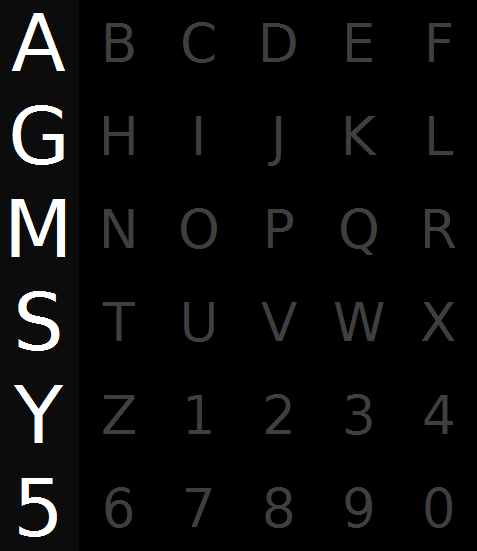
\includegraphics[width=0.35\linewidth]{figs/P300_grid}
% \includegraphics[width=0.65\linewidth]{figs/fig_EEG}
%}
%\caption{(left) The P300 speller grid, using the OpenVibe platform (here the first 
%%column is flashed with some magnification) \cite{Renard10}. (right) 32-channels EEG signal excerpt. 
%Row or column tags are shown on top and stars denotes target row or column (here target row = 6, target column = 8).
%he dashed rectangle indicates an example 600 ms EEG sample taken after flashing the grid at position 8 (2nd column).}
%\label{fig:EEG}
%\end{figure}
%In the absence of labels, automatic signal classification must be used
%in order to decipher the P300 (``target'') responses from the non-P300 (``non-target'') responses. 
The problem is then to identify this particular
ERP (the ``oddball'' ERP) in a set of $K$ observations. 
If we note $\underline{\mathbf{x}} = (\boldsymbol{x}_1,...,\boldsymbol{x}_K) \in \mathcal{X}^K$ the set of $K$ observations,
where $\mathcal{X}$ is the feature vectors space, 
the problem is to identify the ``target'' 
within a set having multiple inputs belonging to the ``non-target'' category
and only one input belonging to the ``target'' category. 
This problem can be seen as a one-\emph{among}-all classification problem\footnote{not to be mixed up with the ``one-vs-all'' classification setup.}.
Noting $P^+$ the target vectorial distribution and
$P^-$ the non-target vectorial distribution, we propose the following generative model: 
Each observation $\underline{\mathbf{x}}$ can be seen as the result of a random draw from a uniform 
mixture of $K$ distributions $P_1, ..., P_K$,  
with $P_1 = (P^+,P^-,...,P^-)$, $P_2=(P^-,P^+,P^-,...,P^-)$, ..., $P_K=(P^-,...,P^-,P^+)$,
each $P_k$ standing for a sequence of $K$ independently drawn feature vectors having the $k^\text{th}$ vector for target.
The uniform prior reflects the uniform probability among the target location in the sequence.

%\begin{figure}
%  \centerline{
%  
\includegraphics[width=0.5\linewidth]{figs/oddball}
%  }
%  \caption{The ``\emph{P300-speller}'' classification problem. The input is a set of $K$ observations. From this set, it
%  is known that $K-1$ observations are drawn according to $P^-$, while only one is drawn according to $P^+$. The position of 
%  this ``oddball'' is unknown. The classification problem consists in identifying the position of the oddball (from its own features and/or by 
%  comparison with the others).}
%  \label{fig:oddball}
%\end{figure}

With such uniform priors, the posterior probability of identifying location $k$ as the target, 
given observation $(\boldsymbol{x}_1,...,\boldsymbol{x}_K)$ is 
easily shown from Bayes formula to be:
\begin{equation}
P(k|\boldsymbol{x}_1,...,\boldsymbol{x}_K) = \frac{\frac{P^+(\boldsymbol{x}_k)}{P^-(\boldsymbol{x}_k)}}
                                          {\sum_l \frac{P^+(\boldsymbol{x}_l)}{P^-(\boldsymbol{x}_l)}} 
\end{equation}
In the linear-Gaussian case, where $P^+$ and $P^-$ are multivariate Gaussian distributions of respective mean
$\boldsymbol{\mu}^+$ and $\boldsymbol{\mu}^-$, with shared covariance $\boldsymbol{\Sigma}$, 
the previous formula simplifies to:
\begin{equation}\label{eq:model-free}
 P(k|\boldsymbol{x}_1,...,\boldsymbol{x}_K) = \frac{\exp(\boldsymbol{x}_k \boldsymbol{w}^T)}
                                             {\sum_l  \exp(\boldsymbol{x}_l \boldsymbol{w}^T)}
\end{equation}
where $\boldsymbol{w}$ can be shown to be equal to $(\boldsymbol{\mu}^+ - \boldsymbol{\mu}^-)\Sigma^{-1}$.
The discriminating manifold $\boldsymbol{x}\boldsymbol{w}^T=0$ is similar to the 
manifold obtained in the binary classification problem, the only difference being the number of samples considered (one sample in the binary
classification case, multiple samples in the ``P300-speller'' classification case). 
Despite the categorical nature of the response, the P300-speller classifier is structurally closer to the binary case 
than to the multiclass case. 

%\begin{table}
%  %\begin{footnotesize}
%  \begin{center}
%    \begin{tabular}{|c||c|c|}
%      \hline
%      & {\bf Model-based} & {\bf Model-free (Softmax-linear)} \\
%      \hline\hline
%      Binary  & 
%      $P(1|\boldsymbol{x}) = \frac{1}{1 + \frac{P^-(\boldsymbol{x})}{P^+(\boldsymbol{x})}}$ &
%      $\pi(\boldsymbol{x};\boldsymbol{w}, b) = \frac{1}{1 + exp(- \boldsymbol{x} \boldsymbol{w}^T + b)}$\\
%      \hline
%      ``P300-speller''  & 
%      $P(k|\boldsymbol{x}_1,...,\boldsymbol{x}_K) = \frac{\frac{P^+(\boldsymbol{x}_k)}{P^-(\boldsymbol{x}_k)}}
%                                          {\sum_{\ell} \frac{P^+(\boldsymbol{x}_\ell)}{P^-(\boldsymbol{x}_\ell)}}$ &
%                                     
%      $\pi_k(\boldsymbol{x}_1,...,\boldsymbol{x}_K;\boldsymbol{w}) =  \frac{\exp(\boldsymbol{x}_k \boldsymbol{w}^T)}
%                                             {\sum_\ell  \exp(\boldsymbol{x}_\ell \boldsymbol{w}^T)}$\\
%      \hline
%      Multiclass  &
%      $P(k|\boldsymbol{x}) = \frac{P(\boldsymbol{x}|k)} {\sum_\ell P(\boldsymbol{x}|\ell)}$  &
%      $\pi_k(\boldsymbol{x}; \boldsymbol{w}_1, ..., \boldsymbol{w}_K) = \frac{\exp(\boldsymbol{x} \boldsymbol{w}_k^T)}{\sum_\ell \exp(\boldsymbol{x} \boldsymbol{w}_\ell^T)}$\\
%      \hline
%    \end{tabular}
%    \end{center}
%    \caption{Formal comparison of the ``P300-speller'' posterior with binary and multiclass posteriors, in the model-based and in the softmax-linear model-free cases.}
%    \label{tab:oddball}
%  %\end{footnotesize}
%\end{table}
%  
  
\subsection{Stochastic classifier}

%In model-free approaches, no assumption is made on the underlying distribution 
%governing the input data. Only a parametrized decision rule  $\pi$ is considered, governing the response of the device. 
%In the ``oddball'' classification case, a simple method is to choose the index that maximizes $\boldsymbol{x}_k \boldsymbol{w}^T$,
%where $\boldsymbol{w}$ is the discriminating manifold, obtained for instance by a linear 
%discriminant analysis \cite{Pfurtscheller1997,Krusienski08,Hoffmann08}. 

We consider the reinforcement learning framework, where different responses must be explored at random before the classifier can estimate which of
them is expected to bring the highest reward. 
The response being obtained from a random draw, the rule that determines the probabilities associated to each possible response is
called the policy.
In our case, consistently with eq. (\ref{eq:model-free}), the policy relies on a vector of parameters $\boldsymbol{w}$ 
that is to be compared with every observation vector from the set $\underline{\mathbf{x}}$
through the scalar products $\langle\boldsymbol{w},\boldsymbol{x}_k\rangle$'s
that are expected to be higher when $\boldsymbol{x}_k$ is a target than when it is not.
The actual response $y \in \{1,...,K\}$ is
drawn from a multinomial distribution relying on the ``$\pi$-scores'' (softmax choice):
\begin{equation}
\label{eq:softmax_multi}
 \forall k \in \{1,...,K\}, \pi(\underline{\mathbf{x}},k;\boldsymbol{w}) = \frac {\exp \langle\boldsymbol{w},\boldsymbol{x}_k\rangle}  {\sum_l \exp \langle\boldsymbol{w},\boldsymbol{x}_l\rangle}
\end{equation}
so that that $\pi(\underline{\mathbf{x}},k;\boldsymbol{w})$ is the probability of having $y=k$ given $\underline{\mathbf{x}}$. 

\subsection{Learning problem}
After the response $y$ is drawn out, a scalar $r(\underline{\mathbf{x}},y)$ (the ``reward'') 
is read from the environment. In essence, the reward quantifies the achievement of the current trial.
The reward expectation $E(r)$ represents the global
achievement of the policy, given by
the integral of the rewards obtained for every observation set $\underline{\mathbf{x}}$ 
and every choice $k$, given their probability of appearance: 
%\begin{equation}\label{eq:objective_pg}
$$E(r) = \int_{\mathcal{X}^K}\Big( \sum_{k=1}^{K} r(\underline{\mathbf{x}},k) \pi(\underline{\mathbf{x}},k;\boldsymbol{w}) \Big)p(\underline{\mathbf{x}}) d\underline{\mathbf{x}}$$
%\end{equation}
where the distribution $p(\underline{\mathbf{x}})$ is not explicitely given. 
The objective is to find the best parameters $\boldsymbol{w}$ for the policy
to maximise the reward expectation, i.e.:
%\begin{equation}\label{eq:optim_pg}
$\max_{\boldsymbol{w}} E(r)$. 
%\end{equation}
We additionally consider a regularization term that
is expected to promote a small norm for the model and priorize
the most recently seen examples in an online setup \cite{Kivinen08}. % (as proposed by ). 
The optimization problem becomes:
\begin{equation}\label{eq:optim_regularized_pg}
  \max_{\boldsymbol{w}} \mathcal{G} = \max_{\boldsymbol{w}} E(r)-{\lambda \over 2} \Vert \boldsymbol{w} \Vert^2 
\end{equation}
where $\mathcal{G}$ is the objective function and $\lambda$ the regularization parameter.

%\subsection{Online update}\label{sec:gradient}
In the absence of a model, the solution of eq.~(\ref{eq:optim_regularized_pg}) can be approached 
by trying to cancel the gradient of $\mathcal{G}$
through a stochastic gradient \emph{ascent}.
The policy gradient is a general purpose reward-based algorithm we adapt here to the online 
``P300-speller'' classification case. 
Following \cite{Wil92}, the regularized policy gradient can be shown to obey to: 
%\begin{equation}\label{eq:simple_pg}
%\nabla_f E(r) = E(r \nabla_f \ln(\pi)) 
%\end{equation} 
%and the regularized policy gradient can be shown to be:
\begin{equation}\label{eq:regularized_pg}
\nabla_{\boldsymbol{w}} \mathcal{G} = E(r \nabla_{\boldsymbol{w}} \ln(\pi)) - \lambda  \boldsymbol{w} 
\end{equation} 
Starting from scratch, the update procedure is expected to refine the model trial after trial 
using the local estimator $\boldsymbol{g}(\underline{\mathbf{x}}, y) - \lambda \boldsymbol{w}$,
with
$\boldsymbol{g}(\underline{\mathbf{x}}, y) =  r(\underline{\mathbf{x}},y)\nabla_{\boldsymbol{w}}\ln \pi(\underline{\mathbf{x}},y;\boldsymbol{w})$, 
so that the rewards should be maximized in the long run. 
From the derivation of $\ln \pi$ according to $\boldsymbol{w}$, we obtain the following expression:
\begin{equation}\label{eq:pol_grad_multi}
 \boldsymbol{g}(\underline{\mathbf{x}}, y) 
= r(\underline{\mathbf{x}},y) \left(\boldsymbol{x}_y - \sum_k  \pi(\underline{\mathbf{x}},k;\boldsymbol{w})\boldsymbol{x}_k\right)
\end{equation}
The regularized online policy gradient ascent update  
can be defined the following way:
at every time $t$, after reading $\boldsymbol{x}_t$, $y_t$ and $r_t$, increment $\boldsymbol{w}$ 
with $\eta\left(\boldsymbol{g}(\underline{\mathbf{x}}, y) - \lambda \boldsymbol{w}\right)$, where $\eta$ is the \emph{learning rate}, i.e.:
\begin{equationsize}{\small}\label{eq:online_update}
%\begin{equation}
\boldsymbol{w}_t = (1-\eta\lambda) \boldsymbol{w}_{t-1} + \eta r_t \left( \boldsymbol{x}_{y_t,t} 
- \sum_{k=1}^K  \pi(\underline{\mathbf{x}},k;\boldsymbol{w}_{t-1})\boldsymbol{x}_{k,t} \right) 
%\end{equation}
\end{equationsize}

%The sketch of our online learning setup is given in algorithm \ref{algo:sketch}.
%\begin{algorithm}
%\caption{Reward-based online learning}
%\label{algo:sketch}
%\begin{algorithmic}[1]
%\STATE $ \boldsymbol{w} \leftarrow$ initialize\_mapping()
%\LOOP 
%   \STATE $\underline{\mathbf{x}} \leftarrow$ measure\_state()
%   \STATE $y \leftarrow$ choice $(\boldsymbol{w},\underline{\mathbf{x}})$ \hspace{3cm} \emph{see eq. (\ref{eq:softmax_multi})}
%   \STATE $r \leftarrow$ measure\_reward($\underline{\mathbf{x}},y$)
%%   \STATE $\boldsymbol{w} \leftarrow$ update\_mapping($\boldsymbol{w},\underline{\mathbf{x}},y,r$) \hspace{1cm} \emph{see eq. (\ref{eq:online_update})}
%\ENDLOOP
%\end{algorithmic}
%\end{algorithm}

%Every example being presented once and for all, the norm limitation constraint imposes to favour the newest examples 
%against the oldest ones in the update of the parameters \cite{Kivinen08}, so that every shift from the current distribution 
%should be tracked progressively, according to the value of $\eta$ (that can be interpreted as a ``renewal'' parameter). 
%In particular, the product $\eta\lambda$ gives an indication on the number of examples that significantly 
%take part in the classifier build-up (as old examples are progressively erased by more recently
%seen examples). This ``memory span'', that drives the complexity of the classifier, can be 
%approximated to $\frac{1}{\eta \lambda}$, so that
%%between target and non-target, no matter how high or low the scores are,
%%allowing higher values for $\lambda$ (implying a smaller norm to $\boldsymbol{f}$). 
%a smaller $\lambda$ implies a higher ``memory span'' (irrespectively of $\eta$). 



\section{Analysis}\label{sec:analysis}
\subsection{Gradient estimator in the binary reward case}\label{sec:analysis-1}

The policy gradient estimator (\ref{eq:pol_grad_multi}) can be analyzed in the binary reward case, 
i.e when $r(\underline{\mathbf{x}},y)$ takes only two values: $r^+$ when the response is correct and $r^-$ when the response is
incorrect. Using a symmetry argument, we only consider the case $\underline{\mathbf{x}} \in \mathcal{C}_1$, i.e. 
$\boldsymbol{x}_1 \sim P^+$ and $\forall k>1, \boldsymbol{x}_k \sim P^-$, for the analysis.
Considering that $r(\underline{\mathbf{x}},1) = r^+$ and  $r(\underline{\mathbf{x}},k)=r^-$ for k>1,
we have:
$$\boldsymbol{g}(\underline{\mathbf{x}}, y) = (\mathbf{1}_{\{y=1\}} r^+ + \mathbf{1}_{\{y\neq 1\}}r^-) \left(\boldsymbol{x}_y - \sum_k  \pi(\underline{\mathbf{x}},k)\boldsymbol{x}_k\right) $$

Then, noting that:
$$E_{\underline{X},Y}(\boldsymbol{g}) = E_{\underline{X}}\left[E_{Y|\underline{X}}(\boldsymbol{g})\right]$$
we look at the conditional expectation of the gradient
$E_{Y|\underline{X}}(\boldsymbol{g})$,
i.e. we try to estimate the general direction followed when
the set of observations $\underline{\mathbf{x}}$ is given.

Let us introduce few additional notations in order to simplify the writing:
\begin{itemize}
 \item Target: 
    $\boldsymbol{x}^+(\underline{\mathbf{x}}) = \boldsymbol{x}_1 $
 \item Non-targets weighted average : 
    $\boldsymbol{x}^-(\underline{\mathbf{x}}) = \sum_{k>1} \tilde{\pi}(\underline{\mathbf{x}},k) \boldsymbol{x}_k
    \mbox{, with } 
    \tilde{\pi}(\underline{\mathbf{x}},k)=\frac{\pi(\underline{\mathbf{x}},k)}{1 - \pi(\underline{\mathbf{x}},1)}$
 \item Difference (local discriminant vector):
    $\boldsymbol{\Delta}(\underline{\mathbf{x}}) = \boldsymbol{x}^+(\underline{\mathbf{x}}) - \boldsymbol{x}^-(\underline{\mathbf{x}})$. 
\end{itemize}

With some reordering, it can be shown that: %we have shown in section \ref{sec:analysis} that :
\begin{equation}\label{eq:exp_up}
E_{Y|\underline{X}}(\boldsymbol{g}(\underline{\mathbf{x}},y)) = (r^+-r^-) \pi(\underline{\mathbf{x}},1) (1 - \pi(\underline{\mathbf{x}},1)) \boldsymbol{\Delta}(\underline{\mathbf{x}})
\end{equation}
%so that the joint expectation is:
%\begin{equation}
% E_{X,Y}(\boldsymbol{g}(\underline{\mathbf{x}},y)) = (r^+-r^-){E}_X\left[\pi(\underline{\mathbf{x}},1) (1 - \pi(\underline{\mathbf{x}},1)) \boldsymbol{\Delta}(\underline{\mathbf{x}})\right]
%\end{equation}
%which can be compared with (\ref{eq:exp_multi}).
i.e. the local \emph{direction} of the gradient 
is the local discriminant vector $\boldsymbol{\Delta}(\underline{\mathbf{x}})$. 

By principle, as soon as $r^+>r^-$,  the weights update
is expected to promote the correct responses (i.e. those associated with $r^+$). 
Then, remarking that:
$\mathbb{P}(r = r^+|\underline{\mathbf{x}}) =  \pi(\underline{\mathbf{x}},1)$, 
we write:
\begin{align*}
 E_{Y|\underline{X}}(\boldsymbol{g}(\underline{\mathbf{x}},y)) &= \pi(\underline{\mathbf{x}},1) E_{Y|\underline{X}}(\boldsymbol{g}(\underline{\mathbf{x}},y)|r = r^+)\\
&+ (1 - \pi(\underline{\mathbf{x}},1)) E_{Y|\underline{X}}(\boldsymbol{g}(\underline{\mathbf{x}},y)|r = r^-)
\end{align*}
and identify:
\begin{itemize}
  \item[] $E_{Y|\underline{X}}(\boldsymbol{g}(\underline{\mathbf{x}},y)|r = r^+) = r^+ (1 - \pi(\underline{\mathbf{x}},1)) \boldsymbol{\Delta}(\underline{\mathbf{x}})$
  \item[] $E_{Y|\underline{X}}(\boldsymbol{g}(\underline{\mathbf{x}},y)|r = r^-) = - r^- \pi(\underline{\mathbf{x}},1) \boldsymbol{\Delta}(\underline{\mathbf{x}})$
  \end{itemize}

If the response is correct \emph{and} $r^+ > 0$, the gradient direction $\boldsymbol{\Delta}(\underline{\mathbf{x}})$ 
is followed, giving more chance to the correct choice in the next trials.
Interestingly, if the response is incorrect \emph{and} $r- < 0$  (i.e. 
a negative mark is given to wrong choices), the same direction is followed,
so that the chance of making correct choices in the future is also enhanced.
%The \emph{norm} of the gradient is different for correct or incorrect choices, 
%i.e. scaled by $r^+(1-\pi)$ for a correct choice and by $-r^-\pi$
%for an incorrect choice. 
%(i.e. irrespectively of $r^+$ and $r^-$, the more unlikely the response, the higher the norm of the local gradient)
%We have shown that in the binary reward case with $r+ > 0$ and $r^-<0$, 
Each update is thus expected to improve
the rate of correct responses, whether the actual response is correct or not.
%, which provides
%a stronger convergence garanty in comparison with EM-based unsupervised approaches \cite{Li06,Lu09,Kindermans12}.

\subsection{Noise-tolerant learning}\label{sec:non-reliable}
We now consider the case where the reward value is corrupted with a uniform noise $p_\text{valid}$, i.e.  
at each trial, the chance of sending the correct reward is $p_\text{valid}$, the chance of sending the opposite reward is $1-p_\text{valid}$.
Then, the gradient expectation becomes:
\begin{alignsize*}{\footnotesize}
%\begin{align*}
E\left(\boldsymbol{g}(\underline{\boldsymbol{x}},y)\right) =& 
p_\text{valid} (r^+-r^-) E \left[
\pi(\underline{\mathbf{x}},1)(1-\pi(\underline{\mathbf{x}},1))\boldsymbol{\Delta}(\underline{\mathbf{x}}) \right]\\
&+ (1-p_\text{valid}) (r^--r^+) E\left[
\pi(\underline{\mathbf{x}},1)(1-\pi(\underline{\mathbf{x}},1))\boldsymbol{\Delta}(\underline{\mathbf{x}}) \right]\\
=& 
(2 p_\text{valid} -1) (r^+-r^-) E\left[
\pi(\underline{\mathbf{x}},1)(1-\pi(\underline{\mathbf{x}},1))\boldsymbol{\Delta}(\underline{\mathbf{x}}) \right]
%\end{align*}
\end{alignsize*}
In this equation, we recognize the typical $(2p_\text{valid}-1)$ term that appears when analyzing algorithms learning from
noisy labels (see, e.g. \cite{Kearns:1998,Denis:2006,Ralaivola:2006}); it
sets the limiting regimen, i.e. $p_\text{valid}>0.5$, where learning can take place. %In the present work, knowing that the incorrect labelling rate
%is lower than 30%, meaning that $p_{valid}>0.5$, we may safely learn from the data we have access to.
%We can then predict the update procedure will fail to improve the classifier as soon as $p_\text{valid} < 0.5$,
%i.e. when the number of misleading rewards 
%overtakes the number of valid rewards. 
Importantly, the norm of the estimator (and thus the 
speed of the learning process) only displays a linear decrease with the rate of misleading rewards, which ensures 
a correct but slowed down convergence even with a significant proportion of reward errors.
  
\section{Numerical experiments}\label{sec:P300}

\subsection{Dataset and preprocessing}\label{sec:preproc}

\begin{figure}
\centerline{
 \includegraphics[width=\linewidth]{figs-copie/fig_EEG}
}
\caption{32-channels EEG signal excerpt. 
Row or column tags are shown on top and stars denotes target row or column (here target row = 6, target column = 8).
The dashed square indicates an example 600 ms EEG sample taken after flashing the grid at position 8 (2nd column).}
\label{fig:EEG}
\end{figure}

The EEG dataset we use comes from a P300 experiment reported in \cite{Maby10}. 
The data consists of 20 files, one file per subject
measuring the brain activity during a P300-speller
experiment where
each subject had to spell out mentally 220 letters. 
%For  trial letter was expected (the ``target symbol'').
For a given letter, rows and columns are flashed in random order
in order to enhance the ``surprise'' when the target row or column
is illuminated.
Each row and each column of the grid 
is flashed several times before taking a decision.
In the considered dataset, each row and column was flashed 5 times per trial.
The stimulus duration was 100 ms, the inter-stimulus interval was also 100ms,
so that the total SOA\footnote{Stimulus Onset Asynchrony.} was 200 ms.
%, where the flash order 

A 32-channels EEG signal was recorded during the whole experiment, sampled at 100 Hz.
% For simplicity as well as for clarity, we made the choice of having as few preprocessing as possible.
% On the contrary to most of the approaches seen in the litterature, we make no feature extraction and directly classify
% our vectors after the following light preprocessing step.
% Each trial is composed of many flashes. 
The whole experiment is divided in sequences of $12 \times 5$  flashes, corresponding to one letter spelling trial.
For each series of 60 flashes,  a 1-20 Hz bandpass filter is applied.
Then for each flash time $t$, a 600 ms subsample $\mathbf{s}_{t:t+600 \text{ms}}$ is taken, 
a common reference average substraction is applied, followed by a channel-by-channel normalization.
Such a sample excerpt is presented on figure \ref{fig:EEG}.
The sample is then vectorized and put in its category $\in {1,...,K}$ (row or column number).
With a 100Hz sampling, the dimension of each  data vector is $32 \times 60 = 1920$.
Then a set of multiple ERP observations is constructed the following way:
For $k \in 1,...,12$, calculate class average $\boldsymbol{x}_k$ and normalize it.
Finally, construct 2 multi-ERP set, i.e. $\underline{\mathbf{x}}^\text{row} = (\boldsymbol{x}_1,...,\boldsymbol{x}_6)$ 
and $\underline{\mathbf{x}}^\text{column} = (\boldsymbol{x}_7,...,\boldsymbol{x}_{12})$.


\subsection{Batch training}\label{sec:batch}


In the standard approach, EEG signal are recorded during a training session and analyzed prior to free spelling 
%Specific features are extracted from the EEG channels, that map to the ERPs (event related potentials) 
%that are expected to take place
% within specific temporal intervals after stimulation.
% , where automatic feature extraction is in general combined
%with expert knowledge, using harmonic (wavelet) encoding
%\cite{Bostanov04}, 
%ICA \cite{Xu04} or signal/noise models \cite{Blankertz08,Rivet09,Ang12}
%Standard classification methods are then used to construct a binary classifier 
%from the feature vectors, using robust and well-documented  approaches like ,
%linear discriminant analysis (LDA) \cite{Pfurtscheller1997,Krusienski08,Hoffmann08}, 
%or support vector machines (SVM) \cite{Rakotomamonjy08}.
%After training, the interface is used
%without additional intervention.
(i) to construct a spatial filter that recombines the electrodes
in order to enhance the P300 signal (e.g. xDAWN filter \cite{Rivet09}) and 
(ii) to build a classifier from the filtered data (e.g. LDA \cite{Krusienski08} or Na\"ive Bayes \cite{Ang12,Maby10} classifiers).
Once the spatial filter is determined,
every EEG sample $\mathbf{s}$ is recombined into a \emph{filtered} EEG sample $\mathbf{s}'$,
whose dimension is reduced regarding the initial data,
and used for the batch training of the classifier. 
In the original P300-speller experiment, the training set was composed of
100 trials, and the test set composed of 120 trials.
Here, consistently with our second numerical experiment (section \ref{sec:sp_filt}), we consider a training set of 25 trials only, with 195 trials in the test set.
We verified by cross-validation that both Na\"ive Bayes and LDA classifiers can achieve on average
85\% spelling accuracy  on the test set, which is consistent with state-of-the art results for this number of repetitions.

\subsection{Learning from scratch}

%\paragraph{Cross-validation}
During free spelling, the classifier has to identify in the set of ERPs the index of the row and column where the P300 ERP
took place, so that the resulting letter is at the intersection of this row and this column. 
In a first numerical experiment, learning is made from scratch, without prior information,
i.e. the initial weights vector $\boldsymbol{w}$ is null
and a raw signal is used (no spatial filter).
In order to estimate the improvement of our classifier, we need to run a series of experiments,
record the responses of the classifier
and compare them to the expected ones. 
For a given value of the hyperparameters $\eta$ and $\lambda$, and for every subject, we run 1000 different simulations.
As the \emph{order} of the examples matters in the online classifier build-up,
each simulation corresponds to a different random shuffle of the initial 220 trials.
For each sequence of randomly shuffled letters, we then apply the 
online update (\ref{eq:online_update}), with rewards generated by a simple comparison between the expected
letter %$\boldsymbol{y}^*_t=(y_t^{*,\text{row}},y_t^{*,\text{col}})$ 
and the classifier's response.  
%$\boldsymbol{y}_t=(y_t^\text{row},y_t^\text{col})$, i.e. for $t \in 1,...,220$,
%$$r_t = \mathbf{1}_{\boldsymbol{y}_t=\boldsymbol{y}_t^*} r^+ + \mathbf{1}_{\boldsymbol{y}_t\neq\boldsymbol{y}_t^*} r^-$$
For each subject, the rate of correct spelling is then calculated
(at each trial) as the average over the 1000 experiments.
%\footnote{This 
%specific ``cross-validation'' method is consistent with the online learning methodology, where each training sample is used only once and the 
%update done after each new sample. In particular, there is no separation between a training set and a test set.}. 

\begin{figure}
\centerline{
 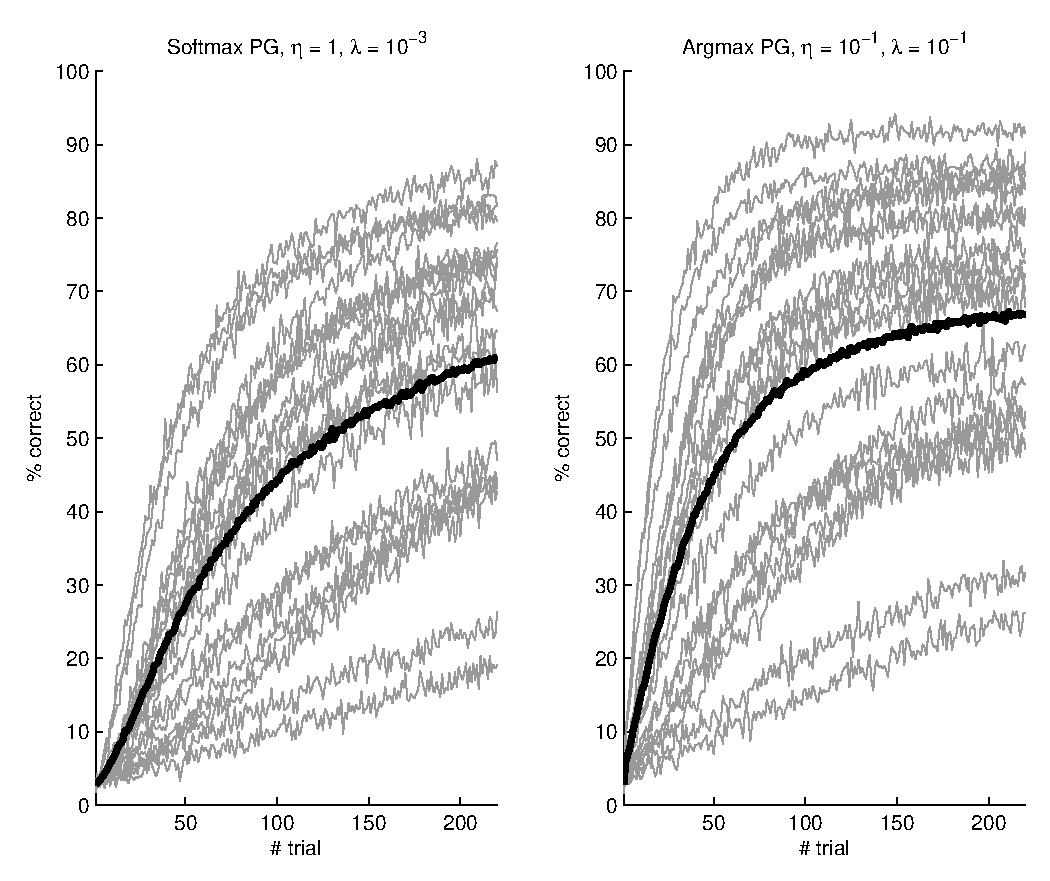
\includegraphics[width=\linewidth]{figs-copie/PG_softmax}
 %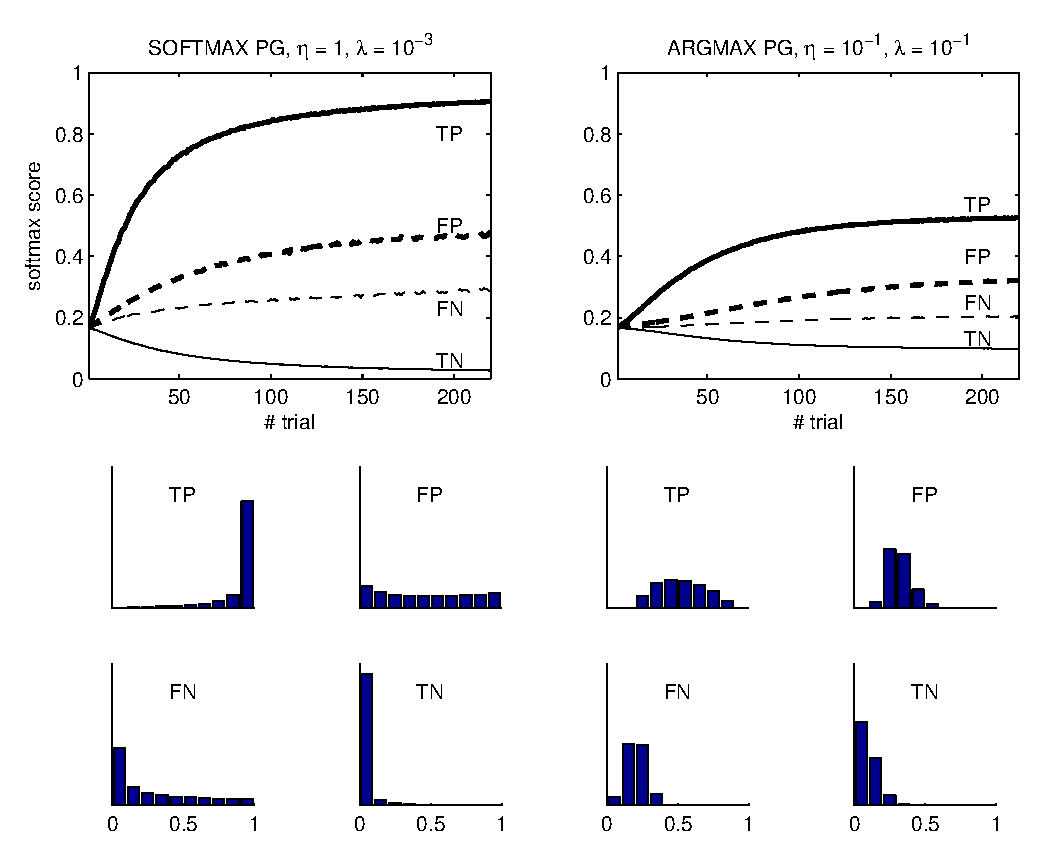
\includegraphics[width=0.5\linewidth]{figs/fig_PG_pi}
}
%\centerline{
%{\bf --~A~--}\hspace{5cm}{\bf --~B~--}
%}
\caption{Spelling improvement during P300-speller experiment (mean over 20 subjects). 
Thin gray lines: Individual improvement. Thick line: Average improvement. 
Left: Softmax policy gradient. Right: Argmax policy gradient. 
%{\bf --~B~--} 
%Softmax scores obtained in the case of true positives (TP), false positives (FP), false negatives (FN) 
%and true negatives (TN). Top: mean $\pi$-score evolution during online learning session, softmax policy gradient (left) and argmax 
%policy gradient (right). Bottom: $\pi$-score distributions at the last trial, softmax PG (left) and argmax PG (right).
}
\label{fig:PG_ref}
\end{figure}

For the rewards, we use the values $r^+ = K-1$ and 
 $r^- = -1$, that can be shown to provide an optimal baseline 
 in the first steps of the gradient ascent (demonstration not given).
%For the dataset
%we have considered, the optimal
%values we obtain are $\eta = 1$ and $\lambda = 10^{-3}$.
%This empirical rate is noted:
%\begin{align*}
%\hat{\rho}_t & = \hat{E}(\mathbf{1}_{\boldsymbol{y}_t=\boldsymbol{y}_t^*}) \\
%       & = \frac{1}{N}\sum_{\text{sim}=1}^N \mathbf{1}_{\boldsymbol{y}_{t,\text{sim}}=\boldsymbol{y}_{t,\text{sim}}^*}
%\end{align*}
%with $r^+ = 5$ and $r^-=-1$.
%\paragraph{Results}
We compare in our experiments two variants of the policy gradient algorithm. 
In a first series, the response $y$ is 
made according to a stochastic ``softmax'' policy, 
and in a second series, it is made according to a deterministic ``argmax'' policy.
In order to fairly compare the two methods, 
we systematically calculate the final spelling accuracy for different values of 
$\eta$ and $\lambda$ ranging from $10^{-5}$ to $10$ using grid search, and find 
markedly different optimal values for
the two cases, i.e. $\eta = 1$ and $\lambda = 10^{-3}$ in the softmax case and
$\eta = 10^{-1}$ and $\lambda = 10^{-1}$ in the argmax case.
%Considering that the norm of $\boldsymbol{w}$ is regulated by 
%the regularization parameter\footnote{the lower $\lambda$, the higher the norm of $\boldsymbol{w}$.}, 
%the higher the difference between the scalar products,
%the more deterministic the choice.
%the lower $\lambda$ (and higher norm of $\boldsymbol{w}$) obtained in
%the softmax case is consistent with a need for contrasted scores, for
%the probabilistic choice to significantly depart from uniformity. On the contrary, in the argmax case, 
%a high contrast is not needed to determine the ``winner''.
%,and the only constraint is to discriminate
%In particular, the product $\eta\lambda$ gives an indication on the number of examples that significantly 
%take part in the classifier build-up (see section \ref{sec:gradient}). 
%This ``memory span'', that drives the complexity of the classifier, can be 
%approximated to $\frac{1}{\eta \lambda}$, so that
%between target and non-target, no matter how high or low the scores are,
%allowing higher values for $\lambda$ (implying a smaller norm to $\boldsymbol{w}$). 
%a smaller $\lambda$ implies a higher ``memory span'' (irrespectively of $\eta$). 

%In the softmax case, the number of examples that allow to reach 
%the final spelling accuracy is found to be O($10^3$), while it is only O($10^2$) in the argmax case. 

We compare in figure \ref{fig:PG_ref} the different learning curves obtained  
in our series of $20 \times 1000$ simulations.
Both average learning curves show a monotonical increase, from $\frac{1}{36}$ (random response)
to an average accuracy of $\simeq$ 60-65\% after 220 trials, with a slight advantage for the argmax case, 
and a tendency toward continuing improvement for $t > 220$.
%This $60\%$ attained in 220 trial can be considered fast,
%since no information except the reward is available to guide the learning process.
Consistently with our expectations (see section \ref{sec:analysis-1}), the steep initial improvement indicates a robust 
gradient following from the very first steps, despite mostly negative rewards 
and occasional misleading rewards (when only the row --~or only the column~-- is correct).
However, despite final slopes suggesting a continuing tendency
toward improvement, the final rates does not attain the 85\% rate obtained in the standard approach 
when combining a spatial filter and a
supervised classifier on a small subset of the training set. 
Moreover, even if a significant improvement is observed for every subject, the inter-subject variability remains quite high, 
with final spelling accuracy peaking to almost 90 \% for the best subjects, but hardly crossing 20\%
for few weaker ones (this discrepancy between subjects being more generally a chronic problem in BCI's). 
Despite its solid converging capabilities, policy gradient from scratch does not appear fast enough when considering
this specific application. We thus consider a more realistic experiment where an initial calibration is followed by an
online improvement procedure.

%\begin{figure}
%\centerline{
% 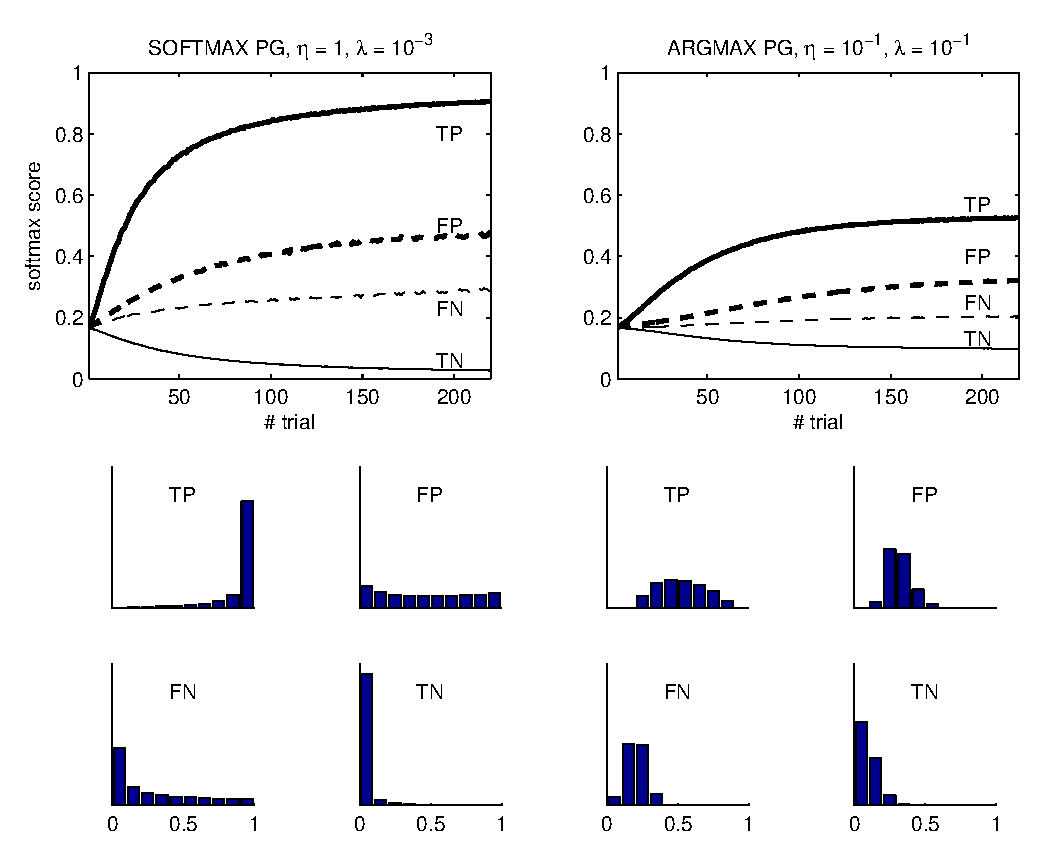
\includegraphics[width=\linewidth]{figs/fig_PG_pi}
%}
%\caption{Softmax scores obtained in the case of true positives (TP), false positives (FP), false negatives (FN) 
%and true negatives (TN). Top: mean $\pi$-score evolution during online learning session, softmax policy gradient (left) and argmax 
%policy gradient (right). Bottom: $\pi$-score distributions at the last trial, softmax PG (left) and argmax PG (right).}
%\label{fig:PG_pi}
%\end{figure}


%We look in figure \ref{fig:PG_pi} at the evolution of the $\pi$-scores obtained in true positives 
%(correct choice), false positives (wrong choice), 
%false negatives (wrong rejection), and true negatives (correct rejection),
%for the softmax choice (left) and the argmax choice (right). 
%Due to a different hyperparameter choice, the separation of the $\pi$-scores is stronger in the softmax case than in the argmax case.
%The main observation here is the significant difference between the $\pi$-score distributions obtained for correct and incorrect 
%choices (or conversely correct or incorrect rejection). 
%The closeness between the false positive and false negative distributions indicate that wrong choices are made 
%when two responses are in close competition. % (two scores are close to 0.5 in the softmax case). 
%The value of the $\pi$-score appears to be a good indicator of the probability of correct response, so that
%the ``confidence'' in the current response could be estimated on the basis of the $\pi$-score value.

\subsection{On-line adaptation} \label{sec:sp_filt}

\begin{figure}
\centerline{
 \includegraphics[width=\linewidth]{figs-copie/fig_filter_2}
}
\caption{xDAWN Spatial filter applied on the EEG signal after a 25 trials training session. The 5 spatial filters (upper bars) define a new
signal that differently combine the initial 32 electrodes. The observation signal is now reduced to 5
channels, each channel having the role of a ``virtual electrode'' (lower figure), where the dashed square indicates 
a 600 ms sample following a flash on column 8 (same sample as in figure 1).}
\label{fig:filter}
\end{figure}

We now consider the classical combination of a spatial filter and a classifier (see sec. \ref{sec:batch}). %, and address the question of
In the previous experiments, the inter-subjects variability remains quite high, 
with weaker subjects hardly reaching 30\% correct spelling rate.
Moreover, the rate attained after 220 trials approaches, but doesn't attain the expected rate of correct spelling
for this data set (around 85 \%), obtained when combining a spatial filter with a
supervised classifier. 
We thus look here how this combination of spatial filter + classifier can be adapted
online in the context of the reward-based approach.
In the following, we note those 
filtered data vectors $\boldsymbol{x}'$ (see figure \ref{fig:filter}).
On the dataset we consider here, this filter training, followed by a classifier training 
%(using formula (\ref{eq:update_logistic_sum}))
allows to reach a rate of correct spelling of 85\% with only 25 trials in the 
training session, which of course challenges the genuine online approach.


\begin{figure}
\centerline{
 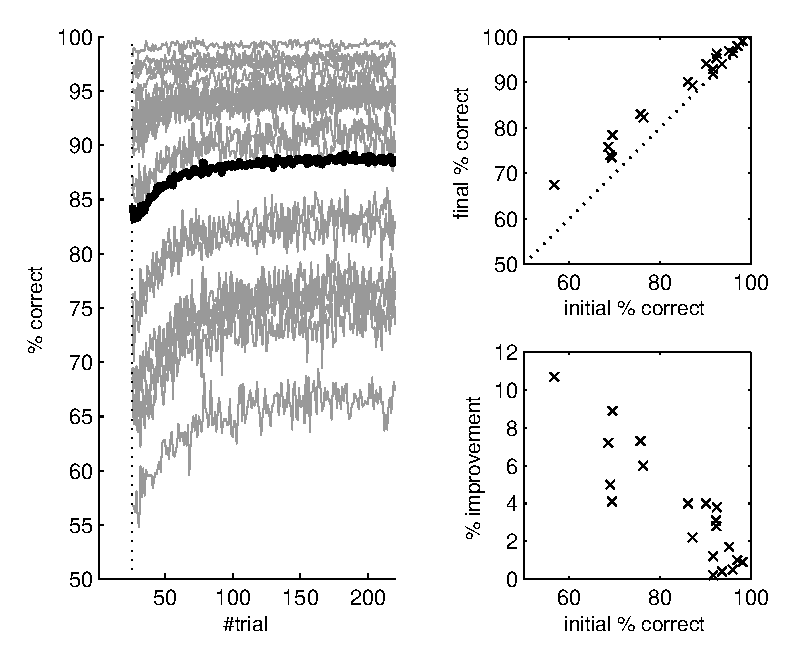
\includegraphics[width=\linewidth]{figs-copie/fig_filter_adapt}
}
\caption{Left: Classification improvement after a 25-trials training session (mean over 20 subjects), 
using linear argmax policy gradient (with $\eta = 10^{-1}$, $\lambda = 10^{-1}$ and $p=5$). 
Thin gray lines: Individual improvement. Thick line: Average improvement. The right figures compare the 
final performance to the initial one, subject by subject, in absolute values (upper right) and in
difference (lower right).}
\label{fig:filter_adapt}
\end{figure}

Then, the online improvement
is done at each trial of the test session (when only rewards are returned to the classifier).
%using formula (\ref{eq:update_multi}).
We present in figure \ref{fig:filter_adapt} the average rate of correct spelling for the trials
following a 25-trials training session. The initial performance (around 85\%) is similar to 
the performance of a standard LDA classifier. Then, a significant improvement is observed, approaching
90\% correct in the last trials of the session.
Interestingly, this improvement can be compared between subjects: The performance improvement
appears negligible for the stronger subjects (around 2 \% when the initial rate is > 80\%) while it
is significantly better (from 6 to 10\%) for subjects whose initiation rate is < 80\%. 
This differential improvement appears interesting for the purpose of reducing the inter-subject
variability, since the weaker subject in our set now attains around 66\% achievement at the end of the session
(while only 56\% at the end of the training). 


\subsection{On-line recovery} \label{sec:sp_filt_rec}

%online adaptation in the context of the reward-based approach.
%\begin{figure}
%\centerline{
% \includegraphics[width=\linewidth]{figs/fig_filter_2}
%}
%\caption{xDAWN Spatial filter applied on the EEG signal after a 25 trials training session. The 5 spatial filters (upper bars) define a new
%signal that differently combine the initial 32 electrodes. The observation signal is now reduced to 5
%channels, each channel having the role of a ``virtual electrode'' (lower figure), where the dashed square indicates 
%a 600 ms sample following a flash on column 8 (same sample as in figure 3).}
%\label{fig:filter}
%\end{figure}
%In the following, we note those filtered data vectors $\boldsymbol{x}'$.
In the non-stationary case, our online adaptive setup requires that both the spatial filter and 
the classifier adapt during  use.
%This co-adaptivity is necessary in case the classifier performance may drop in reason of sudden or progressive
%changes taking place in the EEG signal. Typical example are an electrode that unsticks from the scalp, a progressive change 
%%in electrode conductivity due to long use, or a change in the degree of attention the subject may spend to the task.
In order to test this online recovery capability, we build a specific simulation setup in which we mimic an unexpected 
change taking place at trial number 101. We simply replace the EEG signal from one electrode taken at random 
by a white noise, in order to artificially diminish the rate of successful recognition.
We moreover test the robustness of our approach to erroneous rewards, while manipulating
the rate of misleading rewards, from 100\% valid rewards to only 50\% valid.
At each trial, a random draw is done on the reward reliability $p_\text{valid}$. If a failure is obtained, 
the reward sent to the algorithm is the reverse of what it should be, i.e. $r^-$ instead of $r^+$ and vice versa.

\begin{figure}
\centerline{
 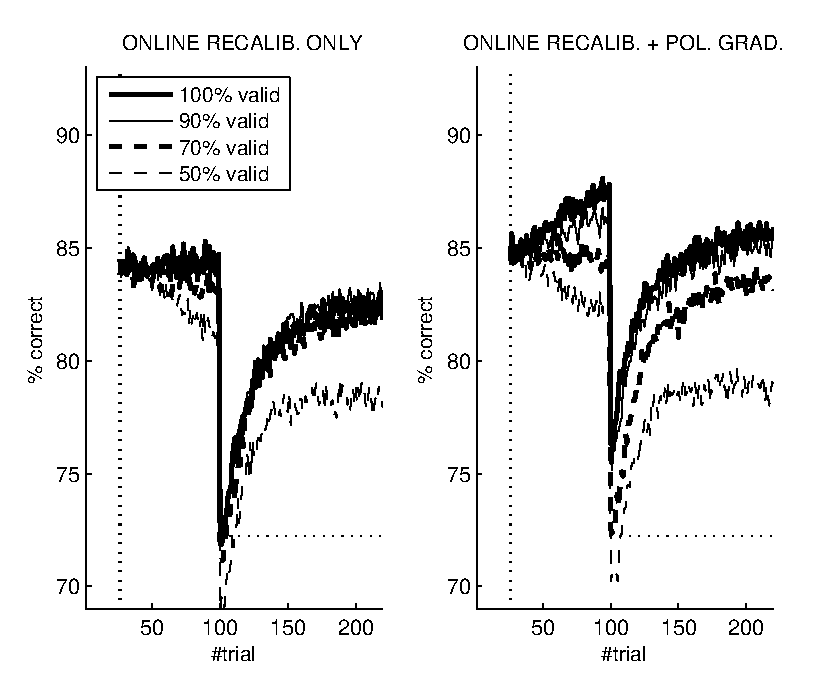
\includegraphics[width=\linewidth]{figs-copie/fig_invalid}
}
\caption{Average spelling rate over 20 subjects, with different reward reliabilities, and electrode break
at trial \# 101. Left: Online recalibration only. Right: Online recalibration + argmax policy gradient.
$\eta = 10^{-1}$, $\lambda = 10^{-1}$. The horizontal dots show the final spelling rate in the absence of 
adaptation.}
\label{fig:invalid}
\end{figure}

Figure \ref{fig:invalid} presents the main results obtained in this setup. The EEG data comes from the same experiment. 
Only the adaptation methods change. 
The left figure presents original results relying on a simple and effective algorithm (called ``reward-based online recalibration'').
In principle, it is possible to recalibrate the device every time a letter is not followed by a backspace, 
which is obviously too resource-consuming. Here we propose to recalibrate the system only when a significant performance drop is observed.
We developed a specific algorithm where (i) a training set, containing only the most recent examples, is maintained during use and 
(ii) the device recalibration is allowed only when the rate of correct spelling is too low (typically 3 successive failures) \cite{Dauce13}.
This algorithm provides a coarse online estimation of the spelling performance, based on the number of failures observed in the three
most recent trials. 
The device update is thus allowed when an unexpected series of three failures is observed.
Only the EEG signal and the labels from the 25 most recent letters for which a positive reward was issued are used to recalibrate the device.   
The figure presents the average correct spelling rates for the trials
following an initial 25-letters training session. The initial performance (around 85\%) is similar to 
the performance of a standard LDA classifier (with this number of repetitions), which of course challenges the genuine online approach
presented in the previous experiment.
The effect of 
a single electrode break (out of 32) appears quite strong, with a big drop from almost 85\% correct to less than
75\% correct.
As expected, a decrease in reward reliability deteriorates the adaptation
and recovery capabilities.
The left figure (online recalibration only) indicates that good recovery capabilities are obtained 
with even 30\% misleading rewards.
Only with 50\% misleading rewards the performance degrades, but still can recover from the artificial electrode breakout,
showing the robustness of the xDAWN filter to false positives (since only positive rewards are
considered in the filter and classifier updates). It is interesting to remark that the sole online recalibration  
seems capable of a recovery up to 78\% correct spelling when half of the rewards are fooling the process. 
This counter-intuitive result can be explained by the fact that in a context of a high correct spelling rate,
most of the false rewards are false negative rewards, whose effect is weaker than the true positives,
as $|r^-|<<|r^+|$ in our setting.

When considering both online recalibration and policy gradient (right figure), a significant improvement is obtained both during the first steps 
following the initial calibration and after the electrode break-out.
This specific effect of the policy gradient is only sensible when the rate of misleading rewards is less than 30\%, otherwise no 
significant improvement is observed.
This can be considered an empirical limit to the policy gradient effectivity in the context of the
P300 speller: If the rate of valid rewards is
less than (or equal to) 70\%, a simple occasional recalibration may be sufficient for online adaptivity to environmental
changes. In the other case,  policy gradient adaptation is worth using in addition to the online recalibration.
This limit is consistent with our theoretical estimate of policy gradient robustness, since the lack of reward reliability may come from 
two distinct causes, namely the 
row and column reward sharing and the reward reliability $p_\text{valid}$ itself\footnote{
For a single row (or column) classification rate $\rho = \sqrt{0.85} \simeq 0.92$, and $p_\text{valid} = 0.7$, 
the effective reward reliability reaches
$(1-\rho+\rho^2) p_\text{valid}\simeq 0.65$, 
which approaches the absolute limit of 0.5 reward reliability we 
stated in section \ref{sec:non-reliable}.
}. 
At last, the combination of policy gradient and online recalibration allows to grab approximately 3\% 
when compared to the sole online recalibration, with a final rate approaching 86\% (to be compared to the 88-89\% 
that can be obtained in the stationary case).
The gain of adaptivity obtained by online recalibration is not at the expense of the improvement
due to the policy gradient. The benefits of the two approaches thus seem to appropriately add up.

%Contrarily to the classifier, the spatial filter is not adaptive since it requires to build a data model 
%on the basis of a training session.
%The data used in the training session can be seen as a
%set of trials $\mathcal{S}$, 
%each trial being composed 
%of an EEG sample $\mathbf{s}$, and its corresponding series of stimuli, and the target row and column 
%given by $\boldsymbol{y}^*$.
%We compare four cases, namely (i) no adaptation, (ii) only policy gradient adaptation, (iii) only spatial filter
%recalibration and (iv) both policy gradient and spatial filter recalibration.

%\begin{figure}
%\centerline{
% 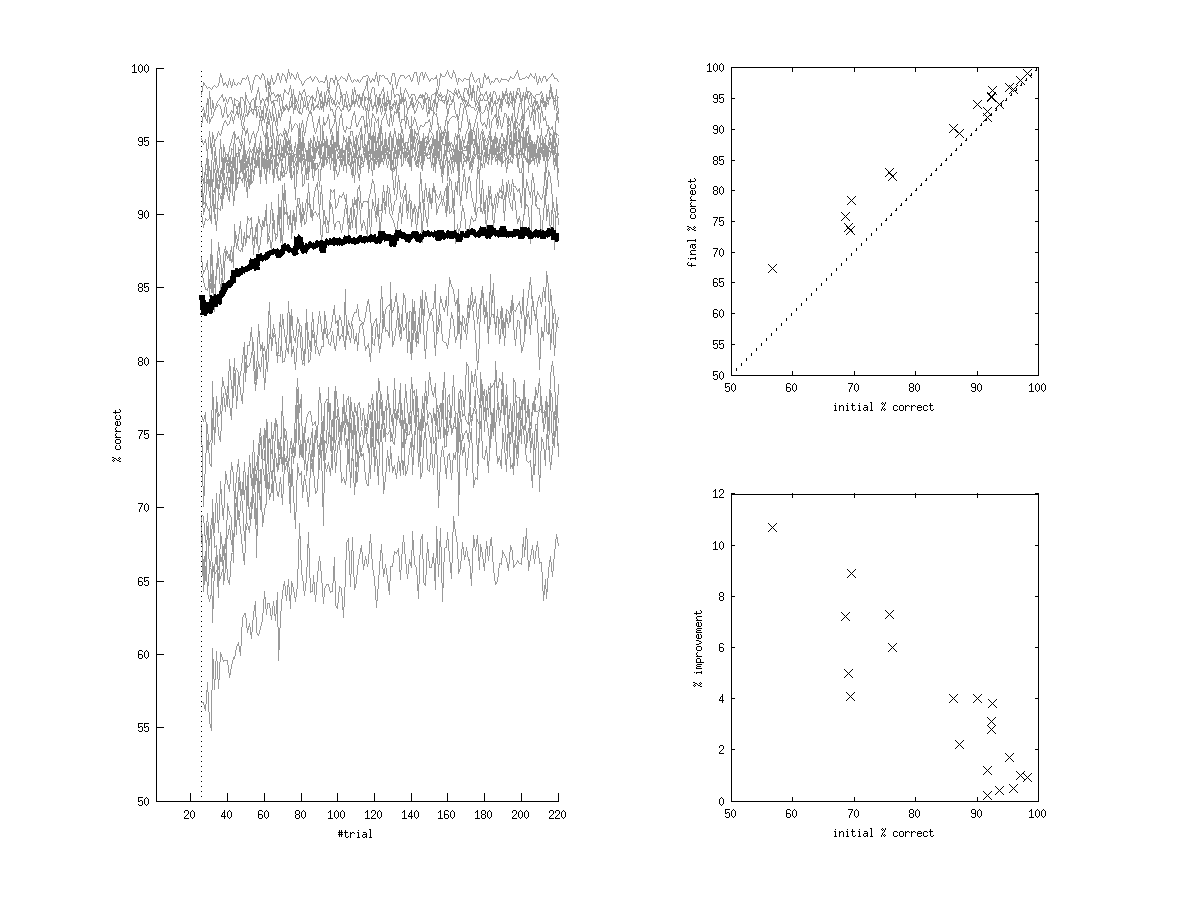
\includegraphics[width=\linewidth]{figs/fig_filter_adapt}
%}
%\caption{Left: classification improvement after a 25-trials training session (mean over 20 subjects), 
%using linear argmax policy gradient (with $\eta = 10^{-1}$, $\lambda = 10^{-1}$ and $p=5$). 
%Thin gray lines: individual improvement. Thick line: average improvement. The right figures compare the 
%final performance to the initial one, subject by subject, in absolute values (upper right) and in
%difference (lower right).}
%\label{fig:filter_adapt}
%\end{figu

\section{Conclusion}

We have presented an application of a policy gradient algorithm 
to the problem of online multi-sample classification, where the multinomial choice means identifying 
the ``oddball'' in a set of $K$ inputs. 
Under this approach, we have shown that every trial should contribute to the classifier improvement, 
provided the return of correct choices is positive and the return of incorrect choices is negative.
We have also given evidence of a good robustness to unreliable rewards 
(when a certain proportion of bad response are erroneously rewarded and/or correct responses 
erroneously dismissed). 
The consistency of our update formula 
has been tested on a P300-speller BCI dataset.
We have considered different experimental conditions. The first experiment (starting from scratch),
has shown the consistency of our update formula with a fast and robust improvement of the 
correct spelling rate in few time steps.
In a second experiment, we have considered the case of the online recovery that is expected to follow 
unforseen events. 
The spelling error information, as typically contained in a backspace hit, has been shown useful for the device adaptivity to unexpected changes. 
Combined with a specific failure detection algorithm, the policy gradient has been shown to appropriately
adapt the classifier to the new situation, at the condition 
the reward is reliable enough (namely having a reliability greater than 70\%).

%Those results are however encouraging for they open perspectives for BCI autonomous online
%improvement, and as such should be used in complement with standard batch classifiers. 

Several perspectives can be opened from this work. First, from a machine learning standpoint, we have
explicited the reward-based online improvement of a random policy (proposed in \cite{Wil92}) to the case of the ``P300-speller'' classifier
with a softmax choice, and drawn 
some correspondences with the ``bandit'' approach \cite{Auer02}. It should be worth at this point to develop a
more thorough comparison with other stochastic exploration methods, and decipher the conditions in which the policy gradient 
is worth using. 
%Second, the stochasticity of non-reliable rewards should be encompassed in the model 
%in order to effectively estimate its impact on variability of the gradient estimator.
Second, from the BCI standpoint, we have shown the feasibility 
of the reward-based approach with a limited feedback.
An interesting possibility would be use a generic classifier (trained for instance from a public P300-speller database) instead of starting
``from scratch''. Provided sufficiently accurate (namely having a spelling accuracy greater than 70\%), a
simple signal like the ``backspace'' key should be enough to robustly improve the speller during use.  


%% The Appendices part is started with the command \appendix;
%% appendix sections are then done as normal sections
%% \appendix

%% \section{}
%% \label{}

%% References
%%
%% Following citation commands can be used in the body text:
%% Usage of \cite is as follows:
%%   \cite{key}          ==>>  [#]
%%   \cite[chap. 2]{key} ==>>  [#, chap. 2]
%%   \citet{key}         ==>>  Author [#]

%% References with bibTeX database:



%% Authors are advised to submit their bibtex database files. They are
%% requested to list a bibtex style file in the manuscript if they do
%% not want to use model1a-num-names.bst.

%% References without bibTeX database:

% \begin{thebibliography}{00}

%% \bibitem must have the following form:
%%   \bibitem{key}...
%%

% \bibitem{}

% \end{thebibliography}

% \appendices
% 
% \section{Symmetry of the gradient expectation}\label{app:exp}
% Considering that 
% \begin{eqnarray*}
% E(\boldsymbol{g}(\underline{\mathbf{x}}, y)) 
% &=&  \sum_k \frac{1}{K} E\left[\boldsymbol{g}(\underline{\mathbf{x}}, y |\underline{\mathbf{x}}\in \mathcal{C}_k)\right]
% \end{eqnarray*}
% 
% we can remark that $\forall k,l$,
% $$
% E\left[\boldsymbol{g}(\underline{\mathbf{x}},y|\underline{\mathbf{x}}\in \mathcal{C}_k)\right] = E\left[\boldsymbol{g}(\underline{\mathbf{x}},y|\underline{\mathbf{x}}\in \mathcal{C}_l)\right]
% $$
% 
% \underline{Proof:} consider $\underline{\mathbf{x}}$ drawn from $P_k$ and take $\underline{\mathbf{x}}^\prime$ 
% the observation matrix drawn from the permutation of columns $k$ and $l$ of $\underline{\mathbf{x}}$. Then:
% \begin{itemize}
%  \item $\underline{\mathbf{x}}\in \mathcal{C}_k \Leftrightarrow \underline{\mathbf{x}}^\prime\in \mathcal{C}_l$ (i.e. $\underline{\mathbf{x}}^\prime$ is drawn according to $P_l$)
%  \item Considering 
% $\boldsymbol{x}_l^\prime = \boldsymbol{x}_k$, $\pi(\underline{\mathbf{x}}^\prime,l) = \pi(\underline{\mathbf{x}},k)$,
% $\boldsymbol{x}_k^\prime = \boldsymbol{x}_l$ and $\pi(\underline{\mathbf{x}}^\prime,k)=\pi(\underline{\mathbf{x}},l)$,
% we verify that  $\boldsymbol{g}(\underline{\mathbf{x}}, y |\underline{\mathbf{x}}\in \mathcal{C}_k) =  \boldsymbol{g}(\underline{\mathbf{x}}^\prime, y |\underline{\mathbf{x}}^\prime\in \mathcal{C}_l)$.
%  \item $E\left[\boldsymbol{g}(\underline{\mathbf{x}}^\prime, y |\underline{\mathbf{x}}^\prime\in \mathcal{C}_l)\right] = E\left[\boldsymbol{g}(\underline{\mathbf{x}}, y |\underline{\mathbf{x}}\in \mathcal{C}_l)\right]$
%  because $\underline{\mathbf{x}}^\prime$ and $\underline{\mathbf{x}}$ obey to the same distribution $P_l$. $\Box$
% \end{itemize}
% 
% \section{Gradient conditional expectation}\label{app:reorder}
% Considering $\mathbb{P}(y=k|\underline{\mathbf{x}}) = \pi(\underline{\mathbf{x}},k)$,
% it comes:
% \begin{align*}
% E_{Y|X}(\boldsymbol{g}(\underline{\mathbf{x}},y)) &= \pi(\underline{\mathbf{x}},1) r^+ \left((1 - \pi(\underline{\mathbf{x}},1)) \boldsymbol{x}_1 - \sum_{k>1} \pi(\underline{\mathbf{x}},k) \boldsymbol{x}_k\right)\\
%                                                              &+ \sum_{k>1}\pi(\underline{\mathbf{x}},k) r^- \left( (1 - \pi(\underline{\mathbf{x}},k))\boldsymbol{x}_k - \sum_{l\neq k} \pi(\underline{\mathbf{x}},l) \boldsymbol{x}_l\right) 
% \end{align*}
% remarking that:
% \begin{align*}
% \sum_{k > 1} \pi(\underline{\mathbf{x}},k) &\left( \boldsymbol{x}_k -  \sum_{l=1}^K \pi(\underline{\mathbf{x}},l) \boldsymbol{x}_l \right)\\
% =& -\pi(\underline{\mathbf{x}},1) \boldsymbol{x}_1 \left(\sum_{k>1}\pi(\underline{\mathbf{x}},k)\right) 
% + \sum_{k>1} \pi(\underline{\mathbf{x}},k)\boldsymbol{x}_k \\
% &-\sum_{l>1} \pi(\underline{\mathbf{x}},l)\boldsymbol{x}_l \left(\sum_{k>1}\pi(\underline{\mathbf{x}},k)\right) \\
% =& - \pi(\underline{\mathbf{x}},1) (1 - \pi(\underline{\mathbf{x}},1)) \boldsymbol{x}_1 + \sum_{k>1} \pi(\underline{\mathbf{x}},k)\boldsymbol{x}_k \\
% &- \sum_{l>1} \pi(\underline{\mathbf{x}},l) \boldsymbol{x}_l 
% + \pi(\underline{\mathbf{x}},1) \sum_{l>1} \pi(\underline{\mathbf{x}},l) \boldsymbol{x}_1\\
% =& - \pi(\underline{\mathbf{x}},1) \left(\boldsymbol{x}_1 - \sum_{k=1}^K \pi(\underline{\mathbf{x}},k) \boldsymbol{x}_k \right)
% \end{align*}
% we obtain:
% %\begin{tiny}
% \begin{align*}
% E_{Y|X}(\boldsymbol{g}(\underline{\mathbf{x}},y)) &= \pi(\underline{\mathbf{x}},1) r^+ \left((1 - \pi(\underline{\mathbf{x}},1)) \boldsymbol{x}_1 - \sum_{k>1} \pi(\underline{\mathbf{x}},k) \boldsymbol{x}_k\right)\\
%                                                              &- \pi(\underline{\mathbf{x}},1) r^- \left((1 - \pi(\underline{\mathbf{x}},1)) \boldsymbol{x}_1 - \sum_{k>1} \pi(\underline{\mathbf{x}},k) \boldsymbol{x}_k\right)
% \end{align*}
% %\end{tiny}


% use section* for acknowledgement
\section*{Acknowledgment}
This research was partly supported by french ANR ``d\'efis'' project CO-ADAPT (ANR-09-EMER-002).
EEG data kindly provided by J\'er\'emie Mattout and Emmanuel Maby from INSERM U1028. 

\bibliographystyle{IEEEtran}
\bibliography{biblio-copie}

\end{document}

%%
%% End of file `elsarticle-template-1a-num.tex'.



